\subsection{Elasticsearch Architecture}
To acheive the scalability across multiple nodes, the final implementation were done in Elasticsearch.
[?? move to approach?]
Elasticsearch has two different mapping options, dynamic mapping and static mapping.

\subsubsection{Elasticsearch Plugin API}
Elasticsearch has it's own plugin API \footnote{\url{https://www.elastic.co/guide/en/elasticsearch/plugins/5.3/index.html}}.
When a plugin is installed, the installation are done on all the nodes.
The plugin API has two main catogories: core plugins and community contributed plugins.
Core plugins are plugins which are a part of the Elasticsearch project.
These plugins are develop by the Elastic team.
Community contributed plugins, are plugins outside the Elasticsearch project.
These plugins are develop by the community.

\subsubsection{Elasticsearch Notes}
- The implementation decribed in this report belongs to the community contributed plugins.

- The implemented plugin extends the current Elasticsearch REST API.

- Architecture with Elasticsearch.

- Elasticsearch plugin to extend the Elasticsearch API.

- Elasticsearch plugin functionality

- Elasticsearch queries in java which are used

\begin{figure}[h!]
\centering 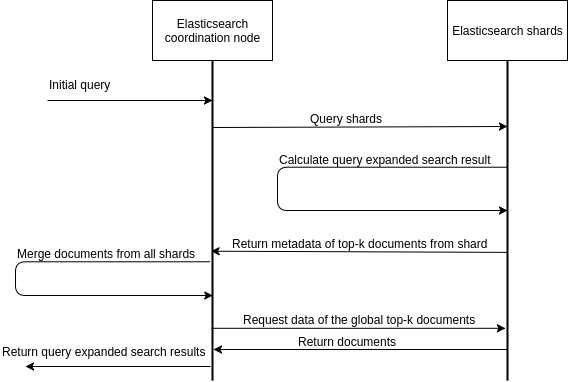
\includegraphics[width=0.9\linewidth]{img/sequence-diagram-elasticsearch.png}
\caption{Sequence diagram for the Elasticsearch implementation.}
\label{fig:sequence-diagram-lucene}
\end{figure}

\subsubsection{Indexing}
\subsubsection{Searching}
